%%%%%%%%%%%%%%%%%%%%%%%%%%%%%%%%%%%%%%%%%
% Arsclassica Article
% LaTeX Template
% Version 1.1 (1/8/17)
%
% This template has been downloaded from:
% http://www.LaTeXTemplates.com
%
% Original author:
% Lorenzo Pantieri (http://www.lorenzopantieri.net) with extensive modifications by:
% Vel (vel@latextemplates.com)
%
% License:
% CC BY-NC-SA 3.0 (http://creativecommons.org/licenses/by-nc-sa/3.0/)
%
%%%%%%%%%%%%%%%%%%%%%%%%%%%%%%%%%%%%%%%%%


%----------------------------------------------------------------------------------------
%	PACKAGES AND OTHER DOCUMENT CONFIGURATIONS
%----------------------------------------------------------------------------------------

\documentclass[
10pt, % Main document font size
a4paper, % Paper type, use 'letterpaper' for US Letter paper
oneside, % One page layout (no page indentation)
%twoside, % Two page layout (page indentation for binding and different headers)
headinclude,footinclude, % Extra spacing for the header and footer
BCOR5mm, % Binding correction
]{scrartcl}

%%%%%%%%%%%%%%%%%%%%%%%%%%%%%%%%%%%%%%%%%
% Arsclassica Article
% Structure Specification File
%
% This file has been downloaded from:
% http://www.LaTeXTemplates.com
%
% Original author:
% Lorenzo Pantieri (http://www.lorenzopantieri.net) with extensive modifications by:
% Vel (vel@latextemplates.com)
%
% License:
% CC BY-NC-SA 3.0 (http://creativecommons.org/licenses/by-nc-sa/3.0/)
%
%%%%%%%%%%%%%%%%%%%%%%%%%%%%%%%%%%%%%%%%%

%----------------------------------------------------------------------------------------
%	REQUIRED PACKAGES
%----------------------------------------------------------------------------------------

\usepackage[
nochapters, % Turn off chapters since this is an article        
beramono, % Use the Bera Mono font for monospaced text (\texttt)
eulermath,% Use the Euler font for mathematics
pdfspacing, % Makes use of pdftex’ letter spacing capabilities via the microtype package
dottedtoc % Dotted lines leading to the page numbers in the table of contents
]{classicthesis} % The layout is based on the Classic Thesis style

\usepackage{arsclassica} % Modifies the Classic Thesis package

\usepackage[T1]{fontenc} % Use 8-bit encoding that has 256 glyphs

\usepackage[utf8]{inputenc} % Required for including letters with accents

\usepackage{graphicx} % Required for including images
\graphicspath{{Figures/}} % Set the default folder for images

\usepackage{enumitem} % Required for manipulating the whitespace between and within lists

\usepackage{lipsum} % Used for inserting dummy 'Lorem ipsum' text into the template

\usepackage{subfig} % Required for creating figures with multiple parts (subfigures)

\usepackage{amsmath,amssymb,amsthm} % For including math equations, theorems, symbols, etc

\usepackage{varioref} % More descriptive referencing

%----------------------------------------------------------------------------------------
%	THEOREM STYLES
%---------------------------------------------------------------------------------------

\theoremstyle{definition} % Define theorem styles here based on the definition style (used for definitions and examples)
\newtheorem{definition}{Definition}

\theoremstyle{plain} % Define theorem styles here based on the plain style (used for theorems, lemmas, propositions)
\newtheorem{theorem}{Theorem}

\theoremstyle{remark} % Define theorem styles here based on the remark style (used for remarks and notes)

%----------------------------------------------------------------------------------------
%	HYPERLINKS
%---------------------------------------------------------------------------------------

\hypersetup{
%draft, % Uncomment to remove all links (useful for printing in black and white)
colorlinks=true, breaklinks=true, bookmarks=true,bookmarksnumbered,
urlcolor=webbrown, linkcolor=RoyalBlue, citecolor=webgreen, % Link colors
pdftitle={}, % PDF title
pdfauthor={\textcopyright}, % PDF Author
pdfsubject={}, % PDF Subject
pdfkeywords={}, % PDF Keywords
pdfcreator={pdfLaTeX}, % PDF Creator
pdfproducer={LaTeX with hyperref and ClassicThesis} % PDF producer
} % Include the structure.tex file which specified the document structure and layout

\hyphenation{Fortran hy-phen-ation} % Specify custom hyphenation points in words with dashes where you would like hyphenation to occur, or alternatively, don't put any dashes in a word to stop hyphenation altogether

%----------------------------------------------------------------------------------------
%	TITLE AND AUTHOR(S)
%----------------------------------------------------------------------------------------

\title{\normalfont\spacedallcaps{Internship report}} % The article title

%\subtitle{Subtitle} % Uncomment to display a subtitle

\author{\spacedlowsmallcaps{Vincent RÉBISCOUL}} % The article author(s) - author affiliations need to be specified in the AUTHOR AFFILIATIONS block

\date{} % An optional date to appear under the author(s)

% ----------------------------------------------------------------------------------------

\usepackage{tikz}
\usepackage{stmaryrd}
\usepackage{amsthm}
\usepackage{algorithm}
\usepackage{algorithmic}

\DeclareMathOperator*{\argmin}{arg\,min}
\DeclareMathOperator{\lcm}{lcm}

\newcommand{\N}{\mathbb{N}}
\newcommand{\V}{\mathcal{V}}
\newcommand{\U}{\mathcal{U}}
\newcommand{\Sp}{\mathcal{S}}
\newcommand{\T}{\mathbb{T}}
\newcommand{\W}{\mathcal{W}}
\newcommand{\Q}{\mathbb{Q}}
\newcommand{\R}{\mathbb{R}}
\newtheorem{defi}{Definition}
\newtheorem{theo}{Theorem}
\newtheorem{lemma}{Lemma}

\begin{document}


%----------------------------------------------------------------------------------------
%	HEADERS
%----------------------------------------------------------------------------------------

\renewcommand{\sectionmark}[1]{\markright{\spacedlowsmallcaps{#1}}} % The header for all pages (oneside) or for even pages (twoside)
%\renewcommand{\subsectionmark}[1]{\markright{\thesubsection~#1}} % Uncomment when using the twoside option - this modifies the header on odd pages
\lehead{\mbox{\llap{\small\thepage\kern1em\color{halfgray} \vline}\color{halfgray}\hspace{0.5em}\rightmark\hfil}} % The header style

\pagestyle{scrheadings} % Enable the headers specified in this block

%----------------------------------------------------------------------------------------
%	TABLE OF CONTENTS & LISTS OF FIGURES AND TABLES
%----------------------------------------------------------------------------------------

\maketitle % Print the title/author/date block

\setcounter{tocdepth}{2} % Set the depth of the table of contents to show sections and subsections only

\tableofcontents % Print the table of contents
\section*{Abstract}
I did my internship at Inria Grenoble,  the subject was:
\textit{"Optimisation avec incertitudes: application à la gestion
  énergétique"} and it lasted 6 weeks. My supervisor was Bruno Gaujal
from  Inria. I had to study a model of the energy consumption of a
processor and then
to work on an improvement of this model. I mainly studied a case where
the processor worked for a fixed amount of time. In a first part, I
will talk about the model the team of the Inria made. Then, in a second
part I will discuss an improvement of the model that I have
made. Finally, I will present a variant of the
problem where the processor works for an indefinite amount of time.\\

Please note that a big part of this report can be found in~\cite{Gaujal}.


\newpage % Start the article content on the second page, remove this if you have a longer abstract that goes onto the second page

\section{A presentation of the problem}
Nowadays, energy consumption is a major issue. Indeed, more power is
more heat which causes a shorter lifetime for the hardware.
Producing electricity is costly and then you need to more money on
cooling and infrastructure which do not come cheap. This is
why my supervisor with Inria has worked on how to minimise the
energy consumption of a processor.

\subsection{A processor consumes energy}
Let say we have a processor that has to do some work. To do it,
the processor can choose several speeds, it can go fast, slow,
intermediate etc... The consumption of energy will depend on the speed
chosen by the processor and the choice of the right speed will be the
core of the problem.
Here, we suppose that energy is a \textbf{convex} function of
the speed, it means that if we want to minimise the energy
consumption, we want to use great speeds as little as possible. We
need to make a mathematical model of a processor that receives tasks
over time and executes them in time. We also want a model that works
online. It means that the jobs are not known in advance by the
processor.\\

We are going to use a Markov Decision Process to
find a policy (a strategy) and
minimise the \textbf{expected} energy consumption by choosing the right
speed. Indeed, MDPs work with probabilities.
Here, we study a case where the processor works until a time
$T\in\N$ (called the time horizon), in our model, the time will be a
finite set
$\{0,1,\dots,T\}$. To represent a job $j_i$, we will need a 3-tuple
$(a_i,s_i,d_i)$ with $a_i\in\N$ the arrival time, in other words, the
time when the job $j_i$ arrives and is acknowledged by the processor. $s_i\in\N$ is the
workload (the ``amount of work''). Finally, $d_i\in\N$ is the deadline
which is the time given to the processor to finish the work,
it means that the job $j_i$ has to be finished before $t=a_i+d_i$. On the
figure~\ref{fig:jobs}, I have represented several jobs: on the x-coordinate
there is the interval in which the work has to be done and on the
y-coordinate there is the workload of the jobs. For example, $j_2$ has an
arrival time $a_2=2$, a workload $s_2=3$ and a deadline
$d_2=4$. Please note that all our variables are natural numbers.\\

\begin{figure}
  \centering
  \caption{Example of jobs}
  \label{fig:jobs}  
  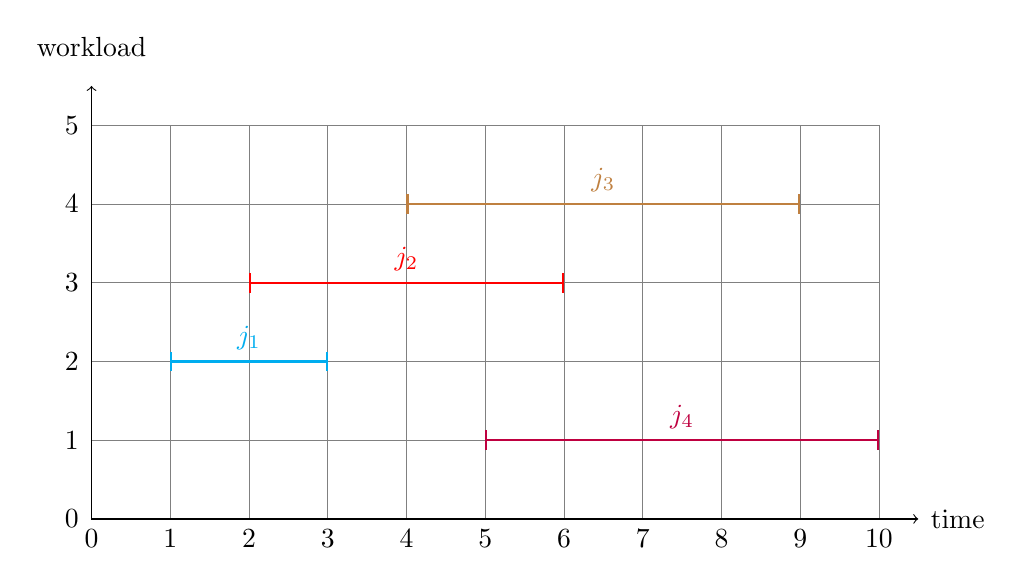
\begin{tikzpicture}
    \draw[help lines] (0,0) grid (10,5);
    \draw[<->] (0,5.5) -- (0,0) -- (10.5,0);
    \foreach \y in {0,1,...,5} \draw (-0.25,\y) node {\y};
    \foreach \x in {0,1,...,10} \draw (\x, -0.25) node {\x};
    \draw (11,0) node {time};
    \draw (0,6) node {workload};
    \draw[|-|,cyan,thick] (1,2) -- (3,2);
    \draw[cyan] (2,2.3) node {$j_1$};
    \draw[|-|,red,thick] (2,3) -- (6,3);
    \draw[red] (4,3.3) node {$j_2$};
    \draw[|-|,brown,thick] (4,4) -- (9,4);
    \draw[brown] (6.5,4.3) node {$j_3$};
    \draw[|-|,purple,thick] (5,1) -- (10,1);
    \draw[purple] (7.5,1.3) node {$j_4$};
  \end{tikzpicture}
\end{figure}

We introduce two parameters: $\Delta$ and $S$ which will be the maximal
deadline and the maximal workload. So, for any job
$j_i=(a_i,s_i,d_i)$, we have $s_i\leq S$, $d_i\leq \Delta$.
The speeds that our processor can choose are represented by a finite
set $\V\subset\N$. To minimise the expected energy consumption, we
need to have some probabilistic information on the jobs that will
come, but we will discuss that later.

\subsection{The remaining work function}
To execute the jobs that the processor has
received, we are going to use the strategy of ``Earliest Deadline
First'', so in priority we do the jobs that needs to be done the
sooner. From there, the only useful information is the workload that
has to be done over time, hence scheduling is not a problem. 
We introduce a function: $D(\cdot)$ where $D(t)$ is the amount of
work that must be done before time $t$. For example, on
figure~\ref{fig:D}, I have represented the function $D(\cdot)$ in
green for the list of jobs of the figure~\ref{fig:jobs}. We can also
define the function $A(\cdot)$ where $A(t)$ is the amount of work that
the processor has received at time $t$, it is represented in red on
figure~\ref{fig:D} The formal definitions of $D(\cdot)$ and $A(\cdot)$
are, if we have $n$ jobs $(a_i,s_i,d_i)$:
\begin{equation}
  \label{eq:D}
  D(t) = \sum_{i=1}^ns_i\times\mathbb{1}_{[a_i+d_i<t]}
\end{equation}

\begin{equation}
  \label{eq:A}
  A(t) = \sum_{i=1}^ns_i\times\mathbb{1}_{[a_i\leq t]}
\end{equation}

Moreover, the function $e(\cdot)$ is represented
where $e(t)$ is the work that has been done at time $t$. So obviously, we
have $D(t)\leq e(t)\leq A(t)$. The slope of the function
$e(\cdot)$ between $t$ and $t+1$ is $v_t\in\N$, the speed of the
processor chosen at time $t$. Please note that at each
$t\in\{0,\dots,T\}$, $e(t)\in\N$. 
The goal  is to find an online
algorithm that finds a function $e(\cdot)$ while minimising the
expected consumption.\\

\begin{figure}
  \centering
  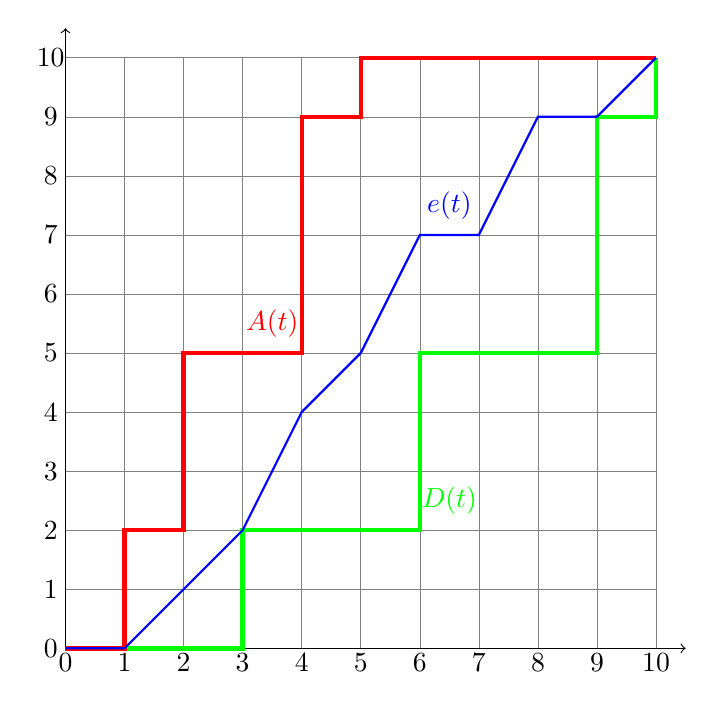
\begin{tikzpicture}[scale=0.75]
    \draw[help lines] (0,0) grid (10,10);
    \foreach \x in {0,1,...,10} \draw (\x,-0.25) node {\x};
    \foreach \y in {0,1,...,10} \draw (-0.25,\y) node {\y};
    \draw[<->] (0,10.5) -- (0,0) -- (10.5,0);
    \draw[green,ultra thick] (0,0) -- (3,0) -- (3,2) -- (6,2) -- (6,5)
    -- (9,5) -- (9,9) -- (10,9) -- (10,10);
    \draw[green] (6.5,2.5) node {$D(t)$};
    \draw[red, ultra thick] (0,0) -- (1,0) -- (1,2) -- (2,2) -- (2,5)
    -- (4,5) -- (4,9) -- (5,9) -- (5,10) -- (10,10);
    \draw[red] (3.5,5.5) node {$A(t)$};
    \draw[blue,thick] (0,0) -- (1,0) -- (3,2) -- (4,4) -- (5,5) -- (6,7) -- (7,7)
    -- (8, 9) -- (9,9) -- (10,10);
    \draw[blue] (6.5, 7.5) node {$e(t)$};
  \end{tikzpicture}
  \caption{Function $D(\cdot)$ and $A(\cdot)$}
  \label{fig:D}
\end{figure}

First, a quick reminder on what a Markov Decision Process is. MDPs are
made to model decision making where the outcome depends on what action
you choose and randomness. For example, I am in location A, I want to
go to location B by taking a cab and I want to go there
\textbf{safely}. I will choose the cab with the well maintained car
but my security will also depend on the sanity of the driver which
will be determined at random. In the end, I will either end up in
location B with probability $p_i$ or at the hospital with probability
$1-p_i$.\\

\begin{figure}
  \centering
 \caption{A example of a MDP}
  \label{fig:mdp}
  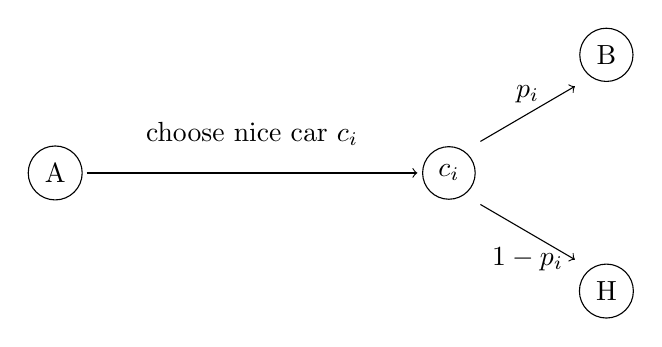
\begin{tikzpicture}
    \draw (0,0) node[circle,draw] {A};
    \draw[->] (0.4,0) -- (4.6,0);
    \draw (2.5,0.5) node {choose nice car $c_i$};
    \draw (5,0) node[circle,draw] {$c_i$};
    \draw (7,1.5) node[circle,draw] {B};
    \draw (7,-1.5) node[circle,draw] {H};
    \draw[->] (5.4,0.4) -- (6.6, 1.1);
    \draw (6,1) node {$p_i$};
    \draw (6,-1.1) node {$1-p_i$};    
    \draw[->] (5.4,-0.4) -- (6.6, -1.1);  
  \end{tikzpicture}
\end{figure}

On figure~\ref{fig:mdp}, from state $A$ we can go to $B$ or to $H$, so our state
space is $\{A,B,H\}$. In our problem, state space will be the space of
the remaining work functions. 
The remaining work at time $t$ is a step increasing function
$w_t(\cdot)$ and $w_t(u)$ is the remaining workload that the processor
has received, that needs to be done before $t+u$. The function $w_t(\cdot)$
only takes into account the jobs that are known by the processor as
opposed to the function $D(\cdot)$
Because all jobs have a deadline bounded by $\Delta$, all $w_t$ are
defined on $\llbracket 0,\Delta\rrbracket$. For example, on figure
\ref{fig:jobs}, suppose we are at $t=2$ and that our processor has not
worked yet. We can see on the graph that $j_1$ and $j_2$ are known by
the processor because $a_1,a_2\leq 2$. Hence the remaining work
function is on figure~\ref{fig:workfun}. The first step represents the
workload of $j_1$ that has to be finished before $t=3$. The second
step represents the workload of $j_2$ that has to be finished before
$t=6$.\\

\begin{figure}
  \centering
  \caption{Remaining work function $w_2(\cdot)$. 
    The red line is the work that has to be done.\\
    Keep in mind that for $w_t(\cdot)$, $w_t(u)$ represents the
  remaining work that has to be done at time $t+u$.}
  \label{fig:workfun}
  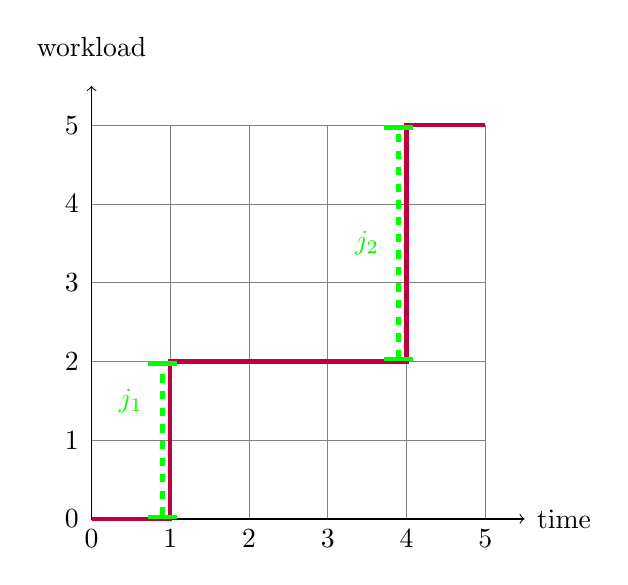
\begin{tikzpicture}
    \draw[help lines] (0,0) grid (5,5);
    \draw[<->] (0,5.5) -- (0,0) -- (5.5,0);
    \draw (6,0) node {time};
    \draw (0,6) node {workload};
    \foreach \x in {0,1,...,5} \draw (\x, -0.25) node {\x};
    \foreach \y in {0,1,...,5} \draw (-0.25,\y) node {\y};
    \draw[purple,ultra thick] (0,0) -- (1,0) -- (1,2) -- (4,2) --
    (4,5) -- (5,5);
    \draw[green,dashed,ultra thick,|-|] (0.90, 0) -- (0.90,2);
    \draw[green] (3.5, 3.5) node {$j_2$};
    \draw[green,dashed,ultra thick,|-|] (3.90, 2) -- (3.90,5);
    \draw[green] (0.5, 1.5) node {$j_1$};    
  \end{tikzpicture}
\end{figure}

The processor works and receives tasks at each
$t\in\{0,1,\dots,T\}$. We suppose the processor can only receive one
job at each step and that fact that no job has arrived at time $t$ is
represented by a job with a workload equals to zero.\\

We will call the space of the remaining work functions $\W$. From state
$w$, which state $w'\in\W$ can we reach ? To know that, we need some
definitions.\\

\begin{defi}
  $\T$ is the shift operator defined as:
  \[ \forall x\in\R,\T f(x) = f(x+1)\]
\end{defi}

\begin{defi}
  $H_t$ is the heavyside function defined as:
  \[ H_t(x) =
    \begin{cases}
      0 & x<t \\
      1 & x\geq t
    \end{cases}
  \]
\end{defi}

\begin{defi}
  $f^+$ is the positive part of function $f$ defined as:
  \[
    \forall x\in\R, f^+(x)=\max(0,f(x))
  \]
\end{defi}

Now, suppose a job $j=(a,s,d)$ arrives at time $t=a$. If the processor
speed at time $t-1$ is $v_{t-1}$ then we have:
\begin{equation}
  \label{eq:nextw}
  w_t(\cdot)=\T[(w_{t-1}(\cdot)-v_{t-1})^+]+s\times H_d(\cdot)
\end{equation}

Once the processor has picked the speed $v_{t-1}$, during one unit of time,
the processor will do $v_{t-1}$ amount of work work so we can
subtract $v_{t-1}$ from
$w_{t-1}$, but the remaining work function must be positive by
definition, hence the term $\T[(w_{t-1}(\cdot)-v_{t-1})^+]$. Then the
term $s\times H_d$ represents the work which was released at time
$t$ and that must be done before time $t+d$.\\

Once the speed at $t-1$ has been chosen, the number of state
accessible is not big, it only depends on what job the processor will
receive at time $t$, in other words, it only depends on the term
$s\times H_d$ in equation~\ref{eq:nextw}.\\

Because deadlines are bounded by $\Delta$ and
workloads by $S$, we have $(S+1)\times\Delta$ possibilities. Indeed, we
have the deadline $d\in\{1,\dots, \Delta\}$ and the workload
$s\in\{0,\dots, S\}$ (the fact that no jobs arrive at time $t$ is
represented by a null amount of work).

\subsection{Finding the right policy}
Now, what we want is to find, given a remaining work function and a
time $t$, what is the right speed to choose to minimise the expected
consumption. But first, we need probabilities about the jobs that can
arrive. We suppose we know $(\phi_w(\cdot,\cdot))_{w\in\W})$ such that:
\begin{equation}
  \label{eq:prob}
  \phi_w(\sigma, \delta)=\Pr(s_t=s,d_t=\delta|w_t=w)
\end{equation}

In other words, $\phi_w(\sigma,\delta)$ is the probability that at state
$w$, a job with a workload $\sigma$ and a deadline $\delta$
arrives. We define $P_v(w,w')$ which is the probability to go to state
$w'$, knowing that at $t-1$ the processor was at state $w$ and at speed $v$.
So we have the equation:
\begin{equation}
  \label{eq:wtowp}
  P_v(w,w')=
  \begin{cases}
    \phi_w(\delta,\sigma) & \mbox{if } w'=\T[(w-v)^+]+\sigma\times
    H_\delta\\
    0 & \mbox{otherwise}
  \end{cases}
\end{equation}

We want a programme which computes a policy given the probabilities
$\phi_w(\cdot, \cdot)$, $S$, $\Delta$ and $T$.
To introduce the algorithm that will allow us to solve the problem, we
need to define two more functions.\\

\begin{defi}
  A policy $\pi(\cdot,\cdot)$ is a function such that
  \[
    \pi:\W\times \{0,\dots,T\}\rightarrow\V
  \]
  For any state $w\in\W$ and $t\in\{0,\dots,T\}$, $\pi(w,t)$ is the
  speed that the processor must choose. This is what we want to
  compute through a programme.
\end{defi}

\begin{defi}
  $J_t(w)$ is the expected consumption given a policy
  $\pi(\cdot,\cdot)$ when at time $t$ and at state $w$.\\
  Formally we have:\\
  \[
    J_t(w)=\mathbb{E}\sum_{s=t}^Tc(\pi(w_s,s))
  \]
  with $w_t=w$
\end{defi}

What we want to find is the optimal policy $\pi^*(\cdot,\cdot)$:
\begin{equation}
  \label{eq:rightpolicy}
  J^*(w_0)=\min_\pi \left(\mathbb{E}\left(\sum_{t=0}^Tc(\pi(w_t,t))\right)\right)
\end{equation}

With $J^*$ being the optimal expected consumption, $w_0$ being the
initial state and $c(v)$ being the consumption of the processor when
going to speed $v$\\

Thanks to the Markov Decision Process Theory, we know the Bellman
equation~\ref{eq:bellman} that we use to compute the right policy.

\begin{equation}
  \label{eq:bellman}
  J^*_t(w)=\min_{v\in\V,v\geq w(1)}\left(
    c(v)+\sum_{w'\in\W}J^*_{t+1}(w')\times P_v(w,w') \right)
\end{equation}

Now we can find the right policy by using the
algorithm~\ref{alg:dpa} which comes from~\cite{Gaujal}.\\

\begin{algorithm}
  \caption{Dynamic Programming Algorithm to find the optimal policy}
  \label{alg:dpa}
  \begin{algorithmic}
    \STATE $t\leftarrow T$
    \FORALL{$w\in\W$}
    \STATE $J_T^*(w)\leftarrow 0$
    \ENDFOR
    \WHILE{$t\geq 1$}
    \FORALL{$w\in\W$}
    \STATE $J_{t-1}^*(w)\leftarrow
    \min\limits_{v\in\V,v\geq
      w(1)}\left(c(v)+\sum\limits_{w'\in\W}P_v(w,w')\times
      J_t^*(w')\right)$
    \STATE $\pi_{t-1}^*(w)\leftarrow
    \argmin\limits_{v\in\V,v\geq
      w(1)}\left(c(v)+\sum\limits_{w'\in\W}P_v(w,w')\times
      J_t^*(w')\right)$
    \ENDFOR
    \STATE $t\leftarrow t-1$
    \ENDWHILE
    \RETURN $\pi^*$
  \end{algorithmic}
  
\end{algorithm}

\begin{lemma}
  The size of the state space is
  \[
    |\W|=\frac{1}{1+S(\Delta+1)}
    \left(
      \begin{matrix}
        (S+1)(\Delta+1) \\
        \Delta+1
      \end{matrix}
    \right)
  \]
\end{lemma}


\begin{theo}
  The complexity of the algorithm is
  \[
    \mathcal{O}(T\times|\V|\times S\times\Delta\times|\W|)
  \]
\end{theo}


Note that the complexity of the algorithm~\ref{alg:dpa} is
exponential. Thankfully, we only have to run the algorithm once offline. It
will compute the right policy $\pi^*$, then any processor will
just have to follow the instructions of the policy and go to speed
$\pi^*(w_t,t)$ when at state $w_t$ and time $t$.

\subsection{My work}

I have implemented the algorithm~\ref{alg:dpa}. The biggest problem
with this algorithm is the complexity of the state space. One can show
that $|\W|=\frac{1}{1+S(\Delta+1)}
    \left(
      \begin{matrix}
        (S+1)(\Delta+1) \\
        \Delta+1
      \end{matrix}
    \right)$
which is exponential. So we needed an algorithm
that computes this set rapidly.\\

The first time I have implemented the programme, I coded in OCaml. The
problem is that OCaml does not handle the multicore yet. You can
use multithreading but the programme will not be able to use several
cores (multithreading is just for concurrency in OCaml). This has
to do with the garbage collector. So I coded pretty much the same
algorithm in C++ to do multithreading. The parallel algorithm works as
follows: the set $\W$ is partitioned in $n$ sets of almost the same size.
\[
  \W=\bigcup_{i=1}^n \W_i
\]
Then, to compute $\pi_{t-1}$ and $J_{t-1}$, one just need $\pi_t$ and
$J_t$, so we parallelized as in algorithm~\ref{alg:dpap} with $id$
being the id of the thread.\\

\begin{algorithm}
  \caption{Dynamic Programming Algorithm to find the optimal policy
    with multithreading}
  \label{alg:dpap}
  \begin{algorithmic}
    \STATE $t\leftarrow T$
    \FORALL{$w\in\W$}
    \STATE $J_T^*(w)\leftarrow 0$
    \ENDFOR
    \WHILE{$t\geq 1$}
    \STATE Launch $n$ threads
    \FORALL{$w\in\W_{id}$} 
    \STATE $J_{t-1}^*(w)\leftarrow
    \min\limits_{v\in\V,v\geq
      w(1)}\left(c(v)+\sum\limits_{w'\in\W}P_v(w,w')\times
      J_t^*(w')\right)$
    \STATE $\pi_{t-1}^*(w)\leftarrow
    \argmin\limits_{v\in\V,v\geq
      w(1)}\left(c(v)+\sum\limits_{w'\in\W}P_v(w,w')\times
      J_t^*(w')\right)$
    \ENDFOR
    \STATE Join the $n$ threads
    \STATE $t\leftarrow t-1$
    \ENDWHILE
    \RETURN $\pi^*$
  \end{algorithmic}
  
\end{algorithm}

My algorithm computes the optimal policy, and then you can simulate a
processor to test it. To compute the optimal policy,
you have to give several parameters like $\Delta, S,T$, the $\V$
set and the probabilities seen in~\ref{eq:prob}.
You can see an example of the simulation on
figure~\ref{fig:simu}. The blue line is the work done by the
processor, while the orange line is the $D(\cdot)$ function. It was
run with the cost function $c(v)=v^2$ and with probabilities
$\phi_w(\delta,\sigma)=\frac{1}{(S+1)\times D}$

\begin{figure}
  \centering
  \includegraphics[scale=0.4]{example_simu.png}
  \caption{Simulation of a processor. Here $T=30,\Delta=4,S=3$}
  \label{fig:simu}
\end{figure}

\subsection{Conclusion}

We have now resolved our problem to minimise the expected consumption
of our processor. But in this model, changing speed is instantaneous. In
reality, this has a cost and my part was to model and make a algorithm
that would take this cost into account.

\section{Generalisation of the problem}

\subsection{Weakness of our model}


The problem with the previous model is that it did not care about the cost of
changing speed. My job was to find a solution. First, we suppose that if
$v_1\neq v_2$, then the time to change speed is $\tau$. It means that
the processor is unable to work during a time $\tau$ like the example
on figure~\ref{fig:delay}.
\begin{figure}
  \centering
  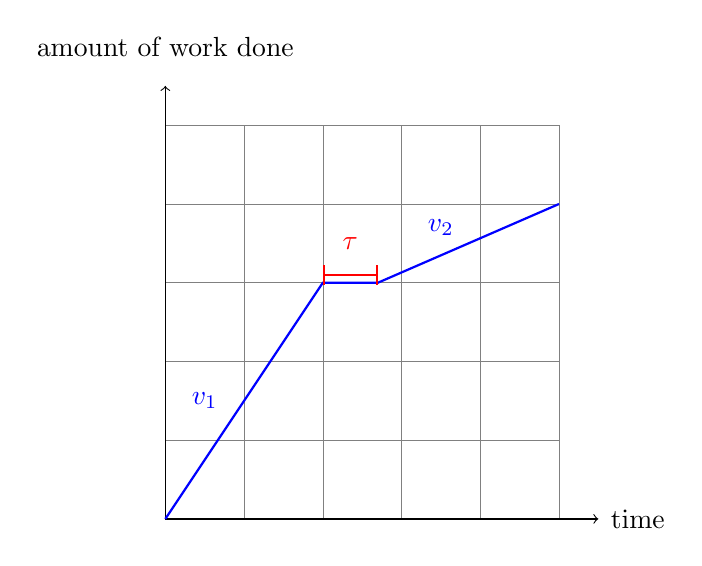
\begin{tikzpicture}
    \draw[help lines] (0,0) grid (5,5);
    \draw[<->] (0,5.5) -- (0,0) -- (5.5,0);
    \draw[thick,blue] (0,0) -- (2,3) -- (2.7,3) -- (5,4);
    \draw (0,6) node {amount of work done};
    \draw (6,0) node {time};
    \draw[blue] (0.5,1.5) node {$v_1$};
    \draw[blue] (3.5,3.7) node {$v_2$};
    \draw[|-|,red,thick] (2,3.1) -- (2.7, 3.1);
    \draw[red] (2.35,3.5) node {$\tau$};
  \end{tikzpicture}
  \caption{$\tau$ delay.}
  \label{fig:delay}
\end{figure}

We want to update our model and to keep it simple too. What we are
going to do is model the change of speed by an over cost. Pay attention
to figure~\ref{fig:overcost}. What we want is to end up in the same
situation that in the model without the cost of changing speed. In the
case $v_1>v_2$ the blue line represents the case where changing speed
costs and the green line represents the standard case. We can see
that, to compensate the lack of work done during a time
$\tau$, we stayed at
speed $v_1$ during a time $\delta$. Because the $c(\cdot)$ consumption function
is convex, this will result in an over cost. Same case for
$v_1<v_2$, note that in that case, the decision to change speed should be
at time $t$ but the processor has changed speed a little before to compensate
the loss of time $\tau$. This is not a problem if we suppose that jobs
are released a little bit before time $t$ so the decision to
change speed can be done sooner.

The value of the over cost is:
\begin{equation}
  \label{eq:overcost}
  f(v_1,v_2)=
  \begin{cases}
    0 & \mbox{if } v_1=v_2 \\
    \delta\times c(v_1) - (\tau + \delta)\times c(v_2)+\tau\times c(0) & \mbox{if }
    v_1>v_2 \\
    \delta\times c(v_2) - (\tau + \delta)\times c(v_1)+\tau\times c(0) & \mbox{if }
    v_1<v_2
  \end{cases}
\end{equation}\\

For the case $v_1>v_2$, we have to subtract $(\tau + \delta)\times
c(v_2)$ because we do not go to speed $v_2$ in the interval
$[t,t+\delta+\tau]$ but we go at speed $v_1$ in the interval
$[t,t+\delta]$ hence we add $\delta\times c(v_1)$. Moreover during
a time $\tau$, the processor does not work so we add some leakage
$\tau\times c(0)$ which can be null.\\

\begin{figure}
  \centering
  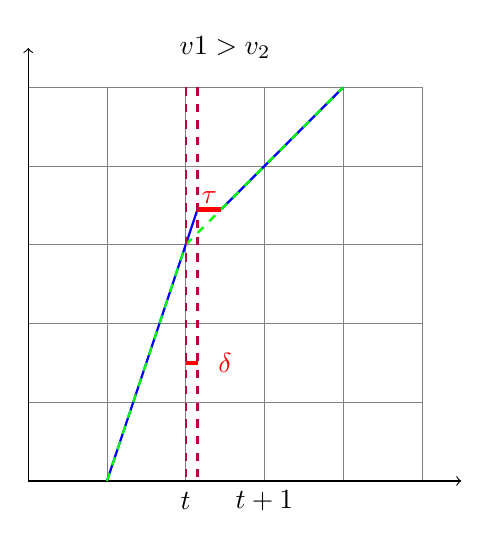
\begin{tikzpicture}
    \draw (2.5, 5.5) node {$v1 > v_2$};
    \draw[help lines] (0,0) grid (5,5);
    \draw[<->] (0,5.5) -- (0,0) -- (5.5,0);
    \draw[blue,thick] (1,0) -- (2.15,3.45);
    \draw[red,ultra thick] (2.15,3.45) -- (2.45, 3.45);
    \draw[red] (2.30, 3.6) node {$\tau$};
    \draw[blue,thick](2.45, 3.45) -- (4,5);
    \draw[green, thick,dashed] (1,0) -- (2,3) -- (4,5);
    \draw (2,-0.25) node {$t$};
    \draw (3,-0.25) node {$t+1$};
    \draw[purple,dashed,thick] (2,5) -- (2,0);
    \draw[purple,dashed,thick] (2.15,5) -- (2.15,0);
    \draw[red] (2.5,1.5) node {$\delta$};
    \draw[red,ultra thick] (2.0,1.5) -- (2.15,1.5);
  \end{tikzpicture}
  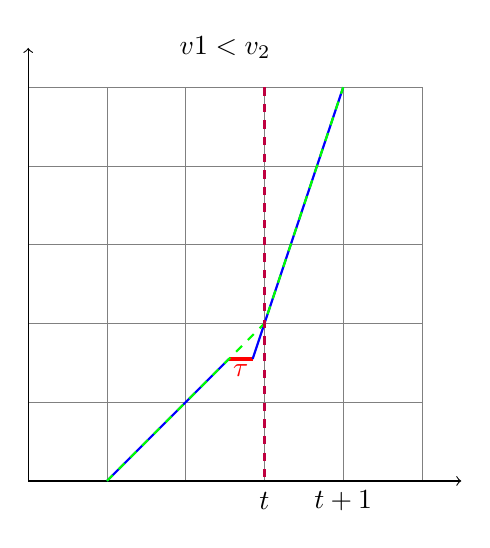
\begin{tikzpicture}
    \draw (2.5, 5.5) node {$v1 < v_2$};
    \draw[help lines] (0,0) grid (5,5);
    \draw[<->] (0,5.5) -- (0,0) -- (5.5,0);
    \draw[blue,thick] (1,0) -- (2.55,1.55);
    \draw[red,ultra thick] (2.55,1.55) -- (2.85,1.55);
    \draw[blue,thick] (2.85,1.55) -- (4,5);
    \draw[green, thick,dashed] (1,0) -- (3,2) -- (4,5);
    \draw[red] (2.70, 1.40) node {$\tau$};
    \draw (3,-0.25) node {$t$};
    \draw (4,-0.25) node {$t+1$};
    \draw[purple,dashed,thick] (3,5) -- (3,0);
  \end{tikzpicture}
  \caption{Change of speed\\
  Green line is the work done in the standard case, blue line is the
  work done in the case with the over cost}
  \label{fig:overcost}
\end{figure}

\begin{lemma}
  Because $c(\cdot)$ is convex, we have $f(v,v')\geq0~\forall v,v'\in\V$.
\end{lemma}


\subsection{The new algorithm}
With some little changes we adapt our algorithm so it will handle
the changing speeds. But first, we need to define $\pi_t^v(w)$ and
$J_t^v(w)$.\\

\begin{defi}
  $\pi$ is a policy and $\pi_t^v(w)\in\V$ is the speed to choose when
  you are at state $w$, time $t$ and your speed at $t-1$ was $v$.\\
\end{defi}

\begin{defi}
  $J_t^v(w)$ is the expected consumption from state $w$ and time $t$,
  knowing that the speed at time $t-1$ was $v$ with policy $\pi$.
\end{defi}

Knowing that, we get our new algorithm~\ref{alg:chgspdalgo}.

\begin{algorithm}
  \caption{Dynamic Algorithm with changing speed}
  \label{alg:chgspdalgo}  
  \begin{algorithmic}
    \STATE $t\leftarrow T$
    \FORALL{$w\in\W,v\in\V$}
    \STATE $J_T^v(w)\leftarrow0$
    \ENDFOR
    \WHILE{$t\geq1$}
    \FORALL{$w\in\W,v\in\V$}
    \STATE $J_{t-1}^v(w)\leftarrow \min\limits_{u\in\V,u\geq w(1)}
    c(u)+f(v,u)+\sum\limits_{w'\in\W}J_t^u(w')\times P_u(w,w')$
    \STATE $\pi_{t-1}^v(w)\leftarrow \argmin\limits_{u\in\V,u\geq w(1)}
    c(u)+f(v,u)+\sum\limits_{w'\in\W}J_t^u(w')\times P_u(w,w')$    
    \ENDFOR
    \STATE $t\leftarrow t-1$
    \ENDWHILE
    \RETURN $\pi^*$
  \end{algorithmic}
\end{algorithm}

\subsection{Results}

\begin{theo}
  The complexity of the algorithm~\ref{alg:chgspdalgo} is
  \[
    \mathcal{O}(T\times|\V|^2\times S\times\Delta\times|\W|)    
  \]
\end{theo}
Once the policy is calculated, you can simulate a processor to
test the results.
The simulator works as follows: you give it the probabilities
$(\phi_{\delta,\sigma})_{1\leq\delta\leq \Delta,0\leq\sigma\leq S}$, a
time horizon $T$ and at for $t=0$ to $T-1$, the
simulator will pick a job with a workload $s$ and deadline $d$
according to $\phi$. Then, the programme computes the new state $w\in\W$
and with the pre calculated policy, the simulator choose the right
speed to use. I also compared the case where you have an over cost and
the case where you do not and you can see it on
figure~\ref{fig:algo_overcost}.\\

\begin{figure}
  \centering
  \includegraphics[scale=0.4]{example_compare.png}
  \caption{Comparison of the work done in standard case (orange line) and the one
    with over cost (blue line). $T=30,\Delta=4,S=3$}
  \label{fig:algo_overcost}
\end{figure}

Unfortunately, the state space is so big that it was hard to test the
algorithm. Only cases with small $S$ and $\Delta$ were tested
(the maximal values tested for $S$ and $\Delta$ were $S=5$ and
$\Delta=5$). On
several cases, we have observed a little trick the processor used to do
one change of speed instead of two as we can see on
figure~\ref{fig:eco} and therefore, making less change of speed which
was exactly the point of this generalisation.

\begin{figure}
  \centering
  \begin{tikzpicture}
    \draw[<->] (0,5.5) -- (0,0) -- (6.5,0);
    \draw[green, thick] (0,0) -- (1,2) -- (3,3.5) -- (6,4.5);
    \draw[blue, thick,dashed] (0,0) -- (1.5,3) -- (6,4.5);
    \draw (1,-0.25) node {$t$};
    \draw[dashed,help lines] (1,0) -- (1,5.5);
    \draw (3,-0.25) node {$t+k$};
    \draw[dashed,help lines] (3,0) -- (3,5.5);
    \draw (6,-0.25) node {time};
    \draw (-1, 5) node {workload};
  \end{tikzpicture}
  \caption{In green the standard case, in blue the advanced case}
  \label{fig:eco}
\end{figure}


\section{Infinite time horizon}

\subsection{The problem}

It is rather rare that the time while a processor works is known in
advance. We can correct that by changing a bit the problem. Now we will try
to minimise the quantity $g^*$ defined as:\\
\begin{equation}
  \label{eq:inftyth}
  g^* = \lim\limits_{T\rightarrow\infty}\sum\limits_{t=1}^Tc(\pi(w_t))
\end{equation}

Note that now, the policy only depends on the current state and that
is exactly what we want. What we are looking for is the optimal
policy, in other words:\\

\begin{equation}
  \label{eq:optpol}
  \pi^*=\argmin_{\pi} \lim\limits_{T\rightarrow\infty}\sum\limits_{t=1}^Tc(\pi(w_t))
\end{equation}

To compute this optimal policy, we use the
algorithm~\ref{alg:inftyth} which comes from the article~\cite{Gaujal}.
I will not get into details because I did
not work on the subject. I only did one implementation. The vector $u$
has a size $|\W|$ because each remaining work function has a slot
written as $u(w)$.\\
\begin{defi}
  If $x$ is a vector then $span(x)=\max_i(x_i)-\min_i(x_i)$\cite{Gaujal}.\\
\end{defi}

\begin{algorithm}
  \caption{Dynamic Algorithm to find a stationary policy}
  \label{alg:inftyth}  
  \begin{algorithmic}
    \STATE $u^0\leftarrow (0,0,\dots,0),~u^1\leftarrow(1,0,\dots,0)$
    \STATE $n\leftarrow1$
    \STATE $\epsilon>0$
    \WHILE{$span(u^n(w)-u^{n-1}(w))\geq\epsilon$}
    \FORALL{$w\in\W$}
    \STATE $u^{n+1}(w)\leftarrow\min\limits_{v\in\V,v\geq
      w(1)}\left(c(v)+\sum\limits_{w'\in\W}P_v(w,w')\times u^n(w')\right)$
    \ENDFOR
    \STATE $n\leftarrow n+1$
    \ENDWHILE
    \STATE Choose any $w\in\W$ and let $g^*\rightarrow
    u^n(w)-u^{n-1}(w)$
    \FORALL{$w\in\W$}
    \STATE
    $\pi^*(w)\in\argmin\limits_{v\in\V,v\geq
      w(1)}\left(c(v)+\sum\limits_{w'\in\W}P_v(w,w')\times
      u^n(w')\right)$
    \ENDFOR
    \RETURN $\pi^*(\cdot)$
  \end{algorithmic}
\end{algorithm}

I implemented the algorithm~\ref{alg:inftyth} and the
convergence time of the algorithm is really small. With
$\Delta=5,S=5$ and $\epsilon=10^{-4}$ it took 1 minutes and 18 seconds
on 4 cores to find the solution when on the case with a time horizon
$T=30$ it took several hours with the same parameters to find the
policy. Unfortunately, I did not have time to study the speed of convergence.


\newpage

\section{Conclusion}
This was my work during my internship at the INRIA. I was able to do
a  nice programme, the biggest I have done for now.
I learned a lot about how to organise my work and be more
productive. Indeed, when I began to implement the algorithm I did not
think enough on a draft so I had to start over some part of the code
several times. One mistake I will make a lot less from now, I am sure.\\

I found the problem I studied really interesting even if I was a bit
frustrated because at the end of the 6 weeks, the questions raised
were the most interesting but I did not have time to think about
it. Thinking of the convergence in the infinite time horizon seemed
really exciting.\\

In this report, I did not talk about some of the work I have tried to
do because it failed. For example, I tried to adapt the code for an
embedded system. I will not get into details but the principle was that a
server had the pre-calculated policy and had to communicate it to a
distant processor with limited memory (so it could not take the whole
policy on its hard drive). I tried to simulate such a process by
coding a server and a client using a TCP/IP connection but my lack of
experience in the domain made my loose a lot of time so I
abandoned.\\

I enjoyed a lot optimisation my algorithms. I worked a lot a trying
different things to gain speed. For example, I use a hash table in my
C++ programme and I had to try several hash functions until I found
something satisfying enough~\ref{sec:hashfun}. This was one of the important work I have
done. I parrallelized my algorithm and it allowed me to compute the 
optimal policy for $S=5,\Delta=5$ so I think it was worth it.\\

\nocite{YaoDS95,Gaujal05}

\bibliographystyle{plain}
\bibliography{biblio}


\newpage

\section*{Appendix A}

I worked in the team Polaris at the Inria Grenoble. Inria is a public
institution dedicated to computational sciences. In the team Polaris I
interacted mainly with my supervisor Bruno Gaujal and a bit with
Nicolas Gast who are two researchers at the Inria. I also dealt with
Annie Simon who is the assistant of the research team Polaris.\\

I was at the IMAG building on the campus of Saint Martin D'Hères,
where there are several laboratories like the Inria but in this
building there are only two teams of this Inria: Polaris and
Datamove. According to inria.fr, there are almost 30 teams of research
on various subjects that exist just in Grenoble.\\

\section*{Appendix B}

I had another idea to model the change of speed but it was less
convenient. Suppose that there is a $\tau\in\Q$ delay to change
speed. $\V\subset\N$, so $\forall v_i\in\V$, $(1-\tau)\times
v_i\in\Q$.\\

\begin{defi}
  \[
    \U=\{(1-\tau)\times v_i~|~\forall v_i\in\V\}
  \]
\end{defi}

We have $\U\subset\Q$ so $\forall u_i\in\U,~u_i=\frac{p_i}{q_i}$ with
$\gcd(p_i,q_i)=1$. We note $m=\lcm(q_i)$ (the least common multiple of
all the denominators). Then $\forall u_i\in\U$, we have $m\times
u_i\in\N$.\\

So by changing $\U:=m\times \U$, we get $\U\subset\N$. We have
computed a set of speeds $\U$ and we can now define:\\
\begin{defi}
  \[
    \Sp=(m\cdot\V)\times \U
  \]
\end{defi}

We have a set of speed but the speeds are $m$ times too big for our
state space $\W$, so we must change that by doing $\W:=m\times
\W$ (we multiply each remaining work function by $m$).
Now, for every $v_i\in m\cdot\V$ we have
$(1-\tau)v_i\in\U$. So we can define the bijection:\\

\begin{defi}
  $\varphi:m\cdot\V\rightarrow\U$ is defined as:
  \[
    \forall v_i\in m\cdot\V,~\varphi(v_i)=(1-\tau)v_i\in\U
  \]
\end{defi}

Suppose we are at speed $v_i$ or $\varphi(v_i)$ between $t$ and $t+1$,
then, at $t+1$, we choose the speed $v_j$ and there are two cases:
\begin{itemize}
\item if $i=j$ then between $t+1$ and $t+2$ we go at speed $v_j$
\item if $i\neq j$ then we go at speed $\varphi(v_j)$
\end{itemize}

But this solution is less practical than the one with an overcost.

\section*{Appendix C}
\label{sec:hashfun}

The hash function I used for my algorithm is:

\begin{defi}
  \[
    h(w) = \sum_{n=1}^\Delta w(n)\times 37^{n-\Delta}
  \]
\end{defi}

\end{document}